\documentclass[12pt]{article}
\usepackage[utf8]{inputenc}
\usepackage{amsmath,setspace,geometry}
\usepackage{amsthm}
\usepackage{amsfonts}
\usepackage[shortlabels]{enumitem}
\usepackage{rotating}
\usepackage{pdflscape}
\usepackage{graphicx}
\usepackage{bbm}
\usepackage[dvipsnames]{xcolor}
\usepackage{hyperref}
\hypersetup{colorlinks=true, linkcolor= BrickRed, citecolor = BrickRed, filecolor = BrickRed, urlcolor = BrickRed, hypertexnames = true}
\usepackage[]{natbib} 
\bibpunct[:]{(}{)}{,}{a}{}{,}
\geometry{left = 1.0in,right = 1.0in,top = 1.0in,bottom = 1.0in}
\usepackage[english]{babel}
\usepackage{float}
\usepackage{caption}
\usepackage{subcaption}
\usepackage{booktabs}
\usepackage{pdfpages}
\usepackage{threeparttable}
\usepackage{lscape}
\usepackage{bm}
%\usepackage[top=15truemm]{geometry}
%\usepackage[]{natbib} 
\bibpunct[:]{(}{)}{,}{a}{}{,}
\setlength{\textwidth}{\paperwidth}     % ひとまず紙面を本文領域に
\setlength{\oddsidemargin}{-5.4truemm}  % 左の余白を20mm(=1inch-5.4mm)に
\setlength{\evensidemargin}{-5.4truemm} % 
\addtolength{\textwidth}{-40truemm}     % 右の余白も20mmに
\renewcommand{\baselinestretch}{0.45}
\newtheorem{proposition}{Proposition}

\setcounter{MaxMatrixCols}{20}

\usepackage{setspace}
\setstretch{1.2}
\begin{document}
\title{Matching Efficiency in the labor markets in Japan, 1966-2024: Nonparametric Approach}
\author{Suguru Otani\thanks{\href{mailto:}{suguru.otani@e.u-tokyo.ac.jp}, Market Design Center, University of Tokyo}}
\maketitle

\begin{abstract}
\noindent
%150 words:
XXX

%100 words AER
\textbf{Keywords}: XXX \\
\textbf{JEL code}: XXX
\end{abstract}

\section{Introduction}

\begin{itemize}
    \item Research question: How has the matching efficiency in the labor market for the unemployed workers changed in Japan in 1966-2024?
\end{itemize}

\begin{itemize}
    \item Japan studies? \cite{fukai2021describing}
\end{itemize}

\section{Data}

I separately use year-level aggregate data in 1966-2023 and month-level aggregate data in 2002 (January)-2024 (April) of the number of job openings, job seekers, and successful job placements, primarily sourced from the Ministry of Health, Labour and Welfare (MHLW) of Japan, which publishes annual reports and statistical data on the Public Employment Security Office, commonly known as Hello Work. 
Hello Work is a government-operated institution in Japan that provides job seekers with employment counseling, job placement services, and vocational training and plays a critical role in Japan's labor market.
For example, \cite{kawata2021first} construct a simple framework to measure the impacts of an economic shock on unemployed workers’ welfare quantitatively and apply their method to Hello Work data in their companion project.\footnote{\url{https://www.crepe.e.u-tokyo.ac.jp/material/crepecl12.html}: Accessed 2024 June 6.}
The period for each dataset is selected to ensure the longest consistent timeframe available at the time of writing this paper.




\section{Model}
Our main interest is in matching efficiency and matching elasticity with respect to the number of unemployed workers and vacancies in the labor market in Japan.
This matching function matters and depends on random search from both sides of the market, that is, individuals seeking jobs represent the supply of labor and recruiters represent the demand for labor.
To estimate the matching function and recover matching efficiency, I follow the novel nonparametric approach proposed by \cite{lange2020beyond}.\footnote{\cite{lange2020beyond} additionally incorporate search effort \citep{mukoyama2018job} and recruitment index \citep{davis2013establishment}. Unfortunately, our Hello Work data does not report the information.}

Let unscripted capital letters $(A, U, V)$ denote random variables while realizations are subscripted by time $t$. 
We consider the matching function $m_t(\cdot,\cdot)$ that maps period-$t$ unemployed workers $U_t$, per-capita search efficacy/matching efficiency of the unemployed workers $A_t$, and vacancies $V_t$ into hires $H_t$.
We assume that the underlying data generating process is stationary and that we observe a long enough time-series so that we can treat the joint distribution $G: \mathbb{R}_{+}^3 \rightarrow[0,1]$ of $\left(H_t, U_t, V_t\right)$ as observed. 
Also, denote by $F(A, U)$ the joint distribution of $A$ and $U$.

We identify the matching function as well as unobserved, time-varying matching efficiency, $A .$ 
First, we assume that $V$ and $A$ are independent conditional on $U$, that is, $A \perp V \mid U$. 
Second, we assume that the matching function $m(AU,V):\mathbb{R}_{+}^2 \rightarrow \mathbb{R}$ has constant returns to scale. 
Then, Proposition 1 of \cite{lange2020beyond} proves that $G(H, U, V)$ identifies $F(A, U)$ and $m(A U, V): \mathbb{R}_{+}^2 \rightarrow \mathbb{R}_{+}$ up to a normalization of $A$ at one point of the support of $(A, U, V)$. Their proof is an application of \cite{matzkin2003nonparametric}.\footnote{\textcolor{blue}{See my companion paper XXX for numerical details. The paper investigates finite sample performance and methodological extension with Monte Carlo simulation. The code is available on the author's Github.}}



\section{Results}

\subsection{Year-level trends in 1966-2023}

For reference, \cite{petrongolo2001looking} summarize the early aggregate studies based on a Cobb-Douglas matching function with the flow of hires on the left-hand side and the stock of unemployment and job vacancies on the right-hand. 
In short, the hire elasticity with respect to unemployment is in the range 0.5–0.7.

Figure \ref{fg:year_level_results}

\begin{figure}[!ht]
  \begin{center}
  \subfloat[Unemployed ($U_{t}$) and Vacancy ($V_{t}$)]{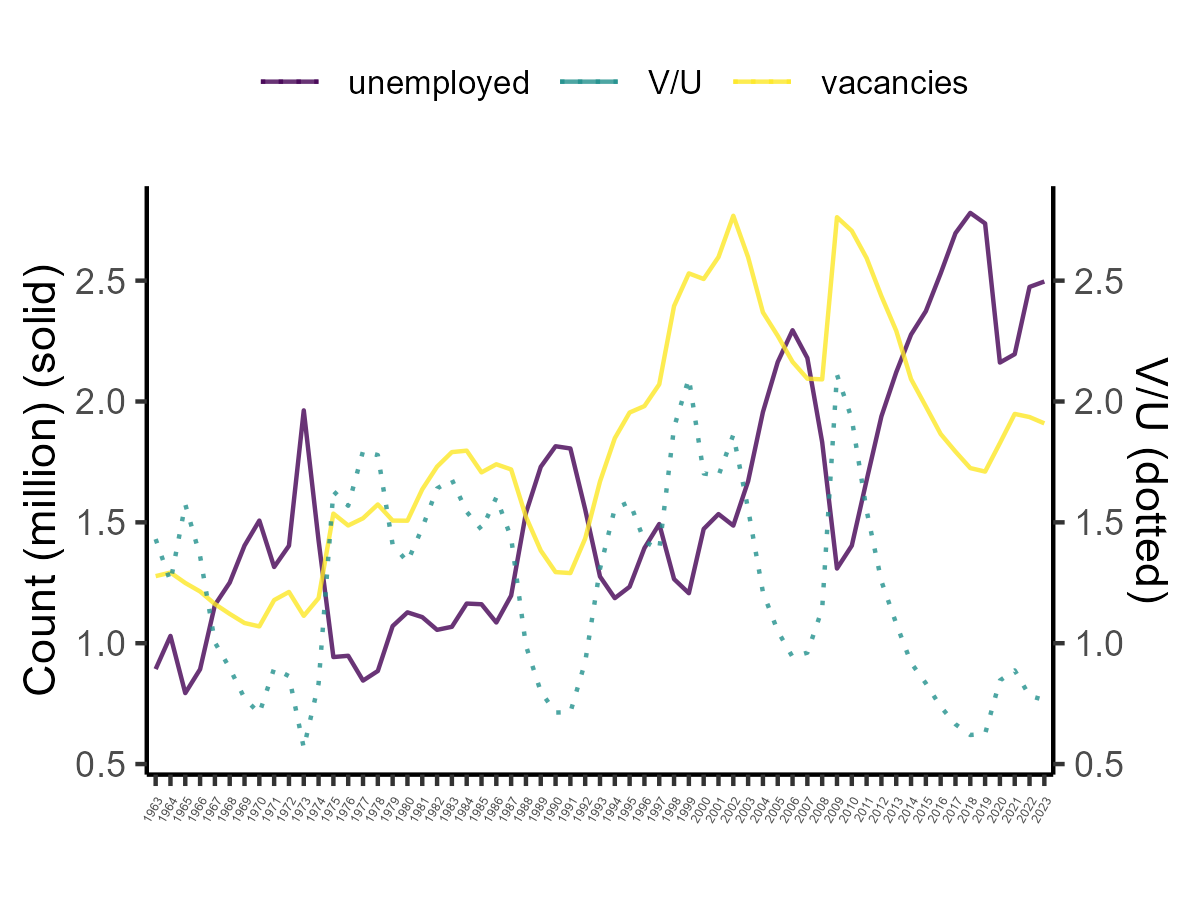
\includegraphics[width = 0.38\textwidth]
  {figuretable/unemployed_vacancy_year.png}}
  \subfloat[Hire ($H_{t}$)]{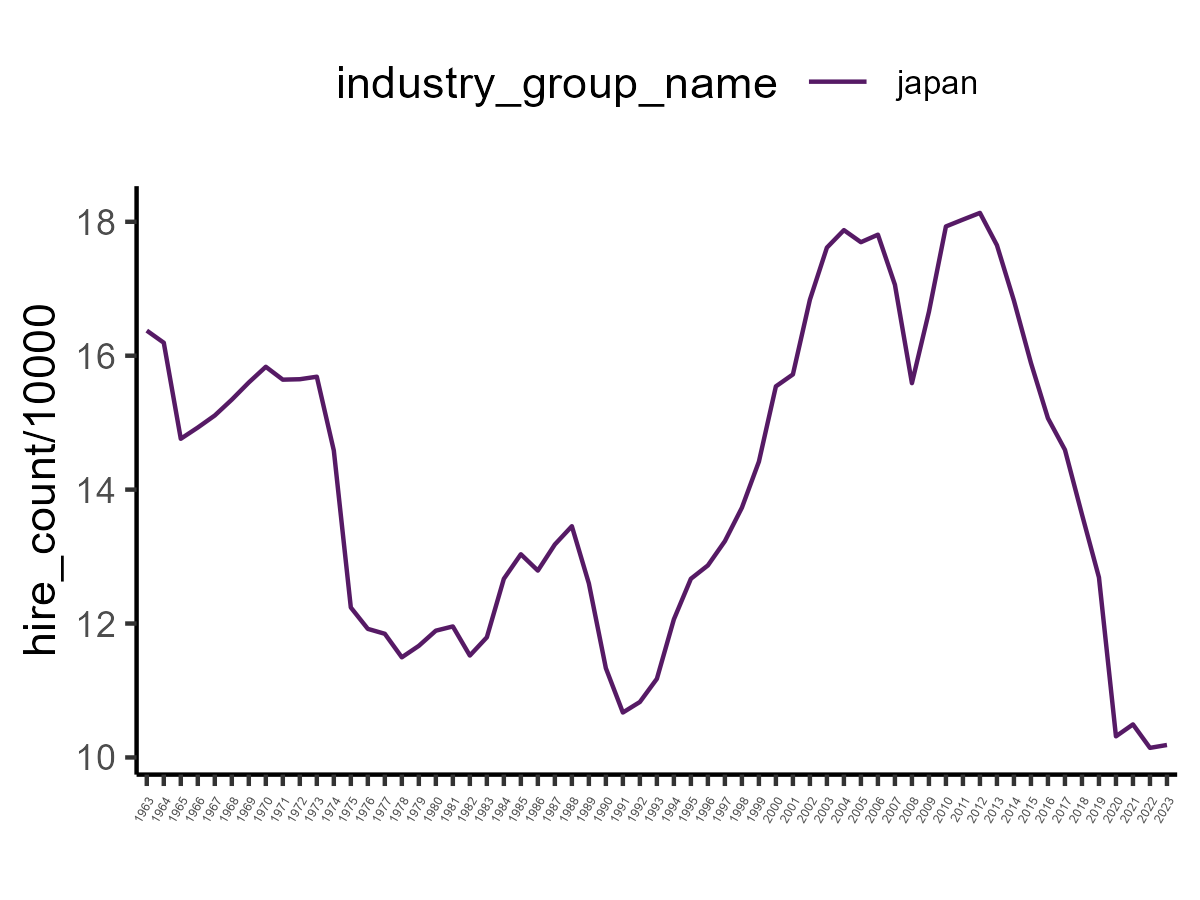
\includegraphics[width = 0.38\textwidth]
  {figuretable/hire_year.png}}\\
  \subfloat[Bevaledge Curve ($U_{t}$ and $V_{t}$)]{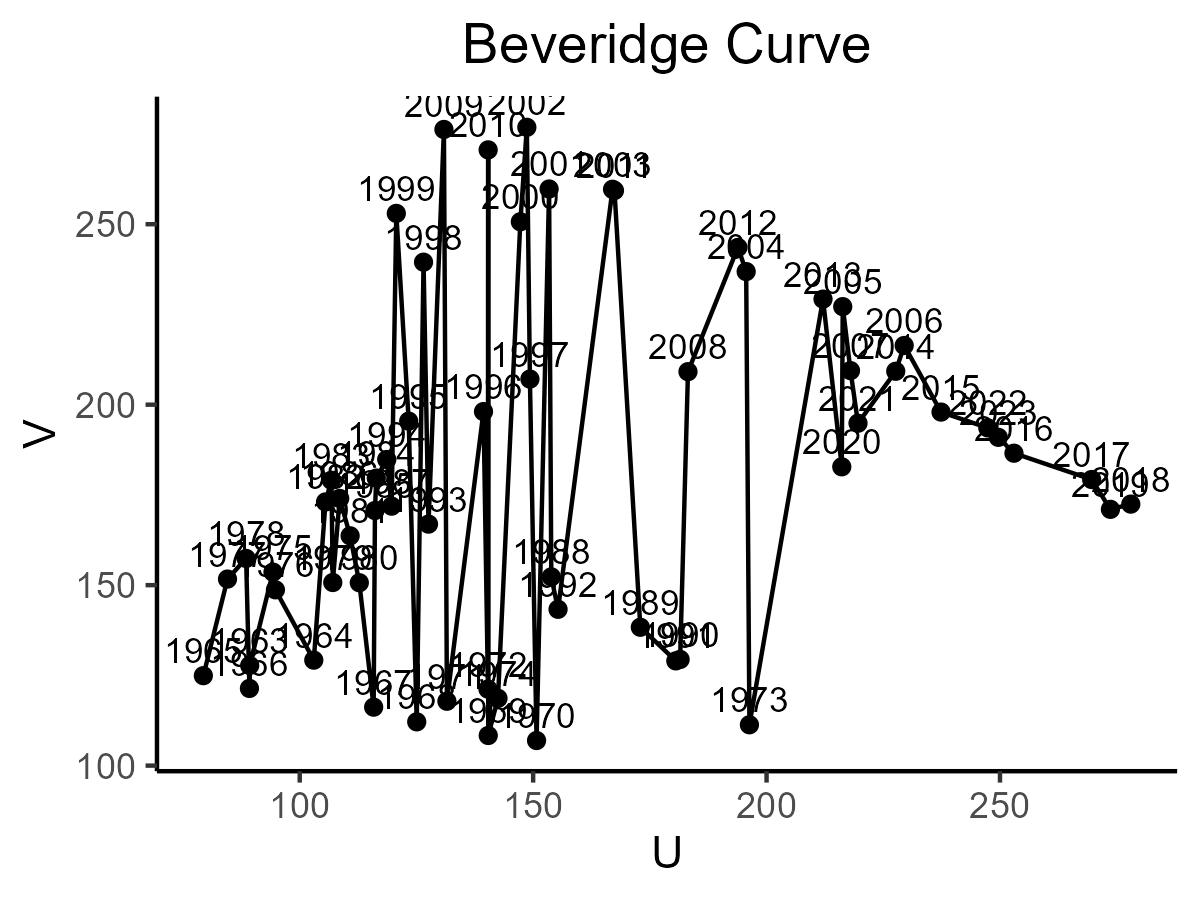
\includegraphics[width = 0.38\textwidth]
  {figuretable/unemployed_vacancies_berveridge_year.png}}
  \subfloat[Log job finding rate and tightness]{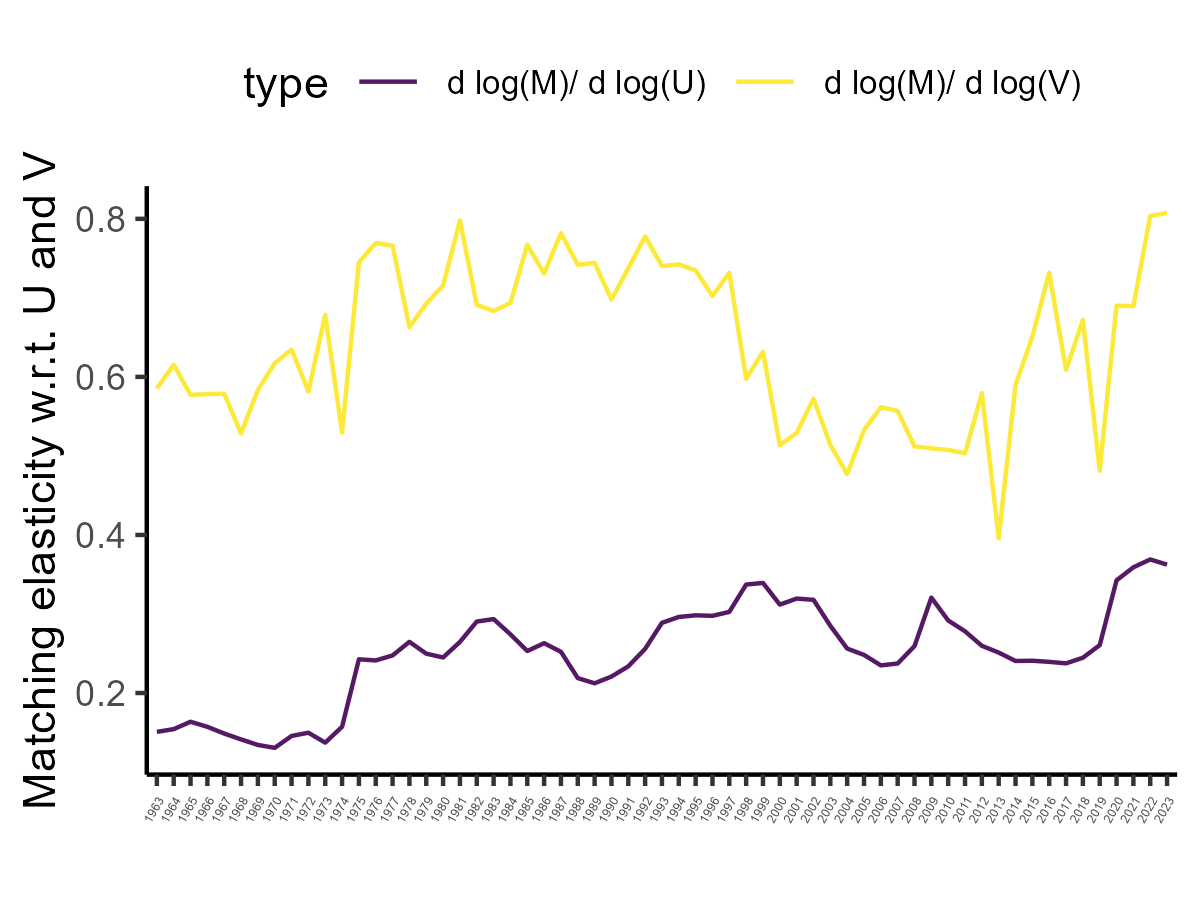
\includegraphics[width = 0.38\textwidth]
  {figuretable/elasticity_year.png}}
  \\
  \subfloat[Matching Efficiency ($A_{t}$)]{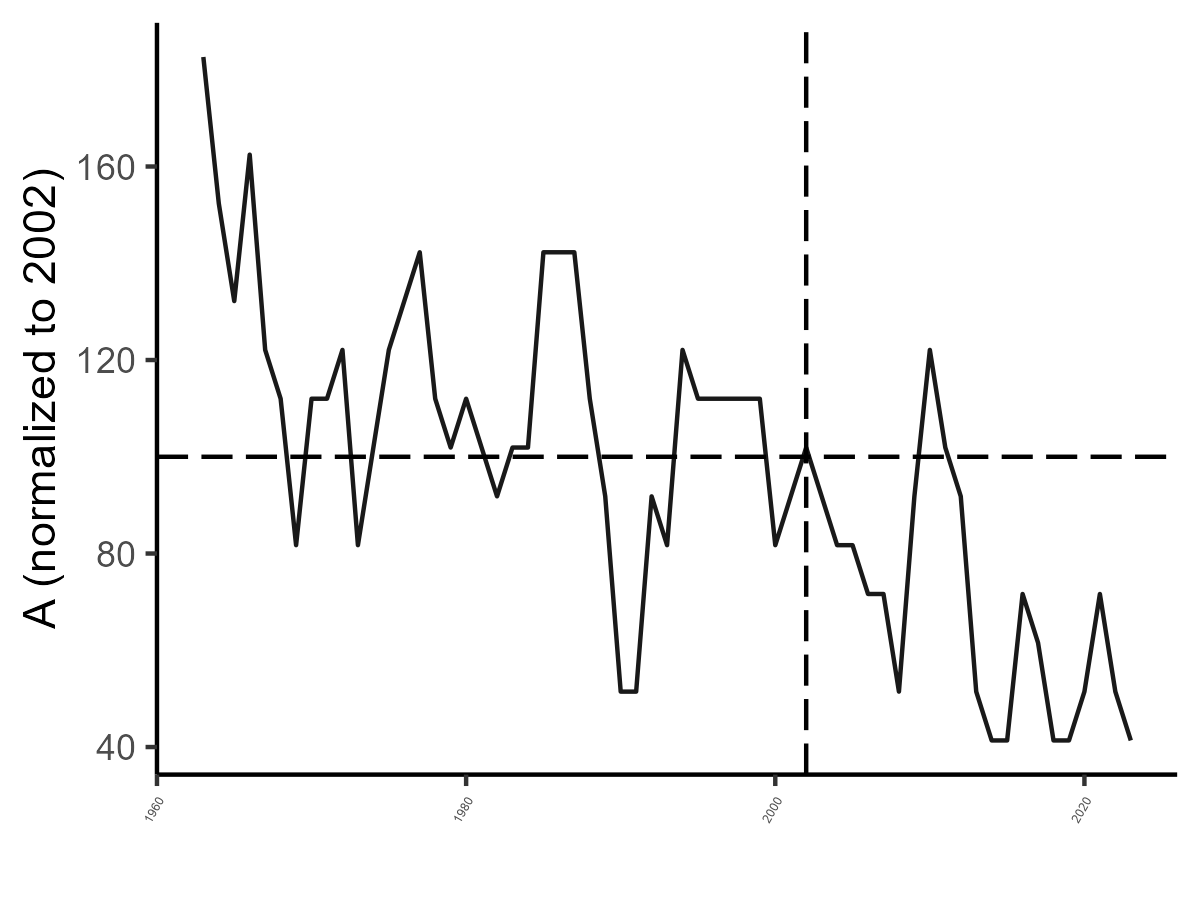
\includegraphics[width = 0.38\textwidth]
  {figuretable/matching_efficiency_year.png}}
  \subfloat[Matching Elasticity ($\frac{dM}{dU}$ and $\frac{dM}{dV}$)]{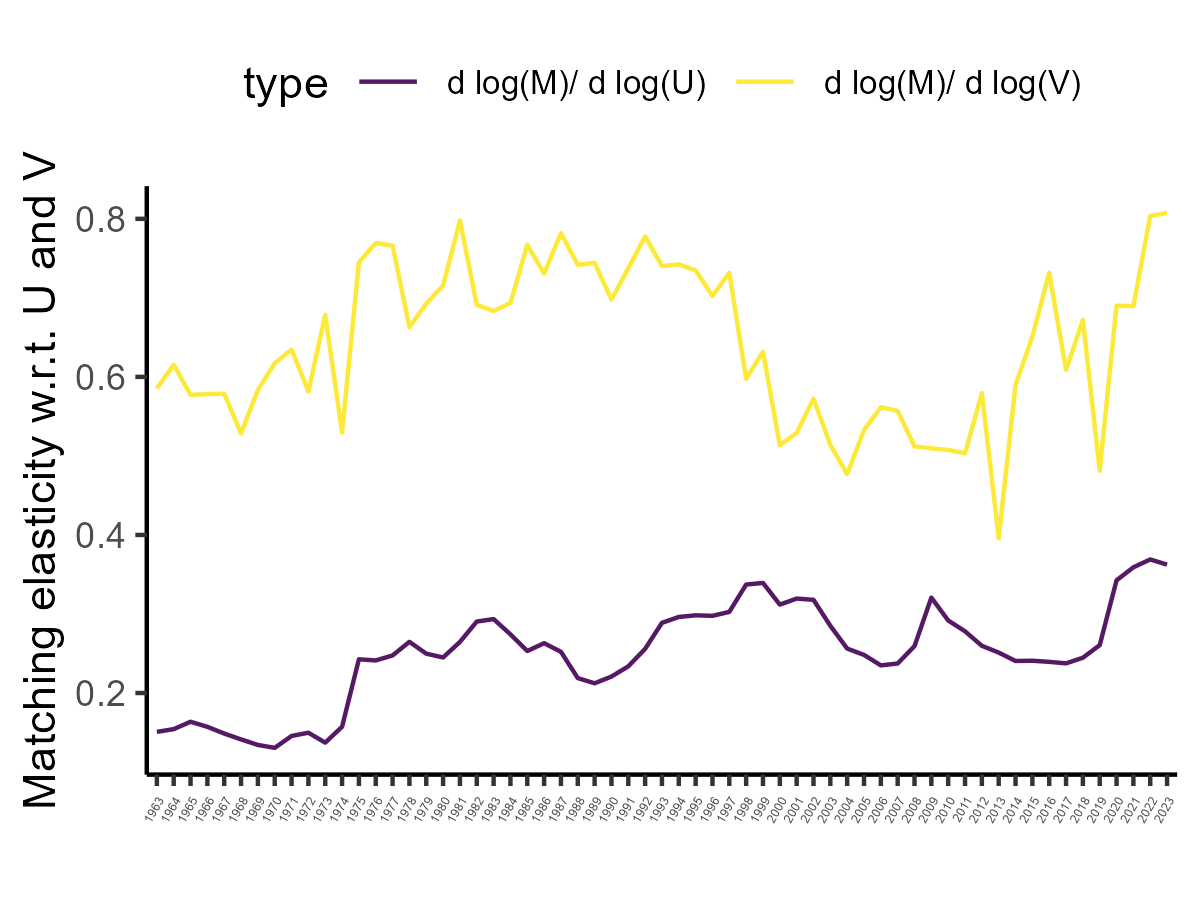
\includegraphics[width = 0.38\textwidth]
  {figuretable/elasticity_year.png}}\\
  \subfloat[Efficiency ($A$) and Tightness ($V/U$)]{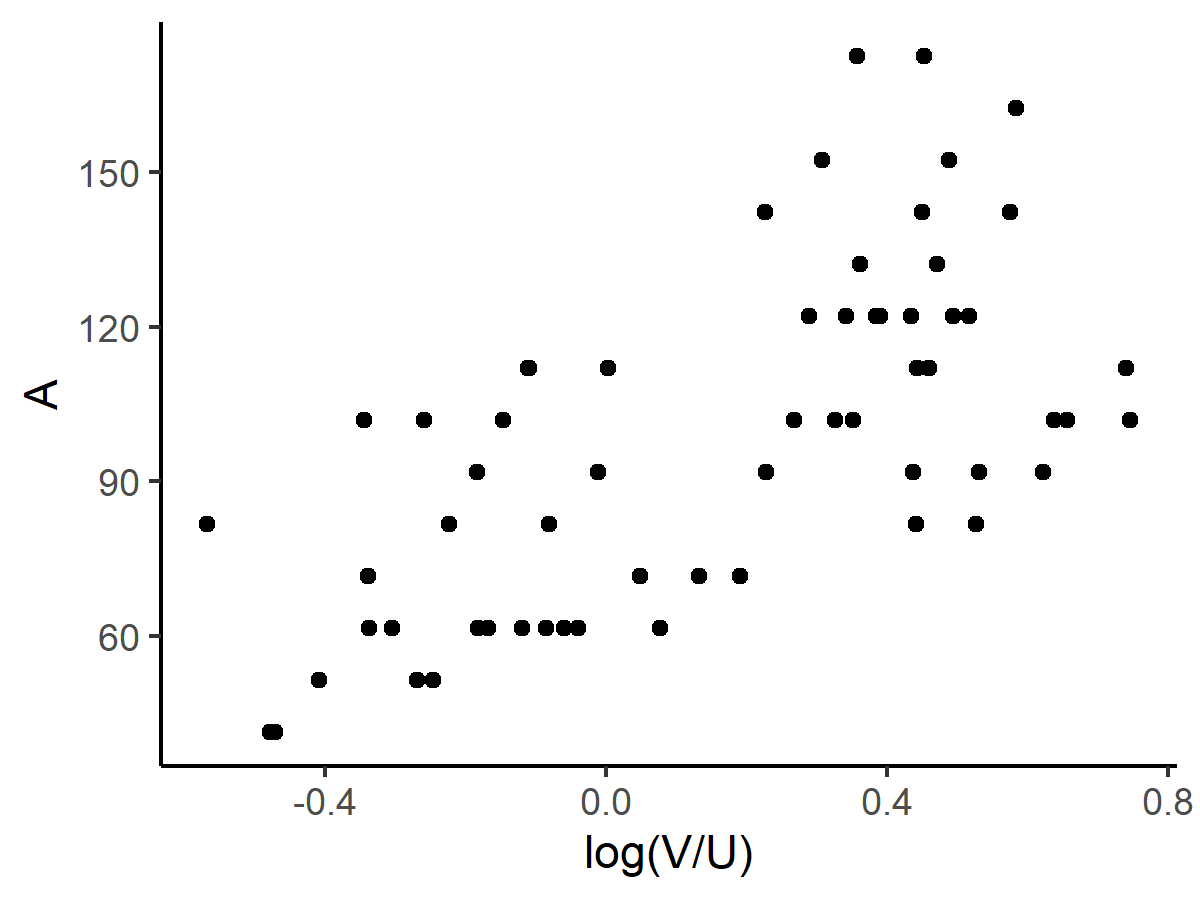
\includegraphics[width = 0.38\textwidth]
  {figuretable/efficiency_tightness_plot_year.png}}
  \subfloat[Efficiency ($A$) and job finding rate ($M/U$)]{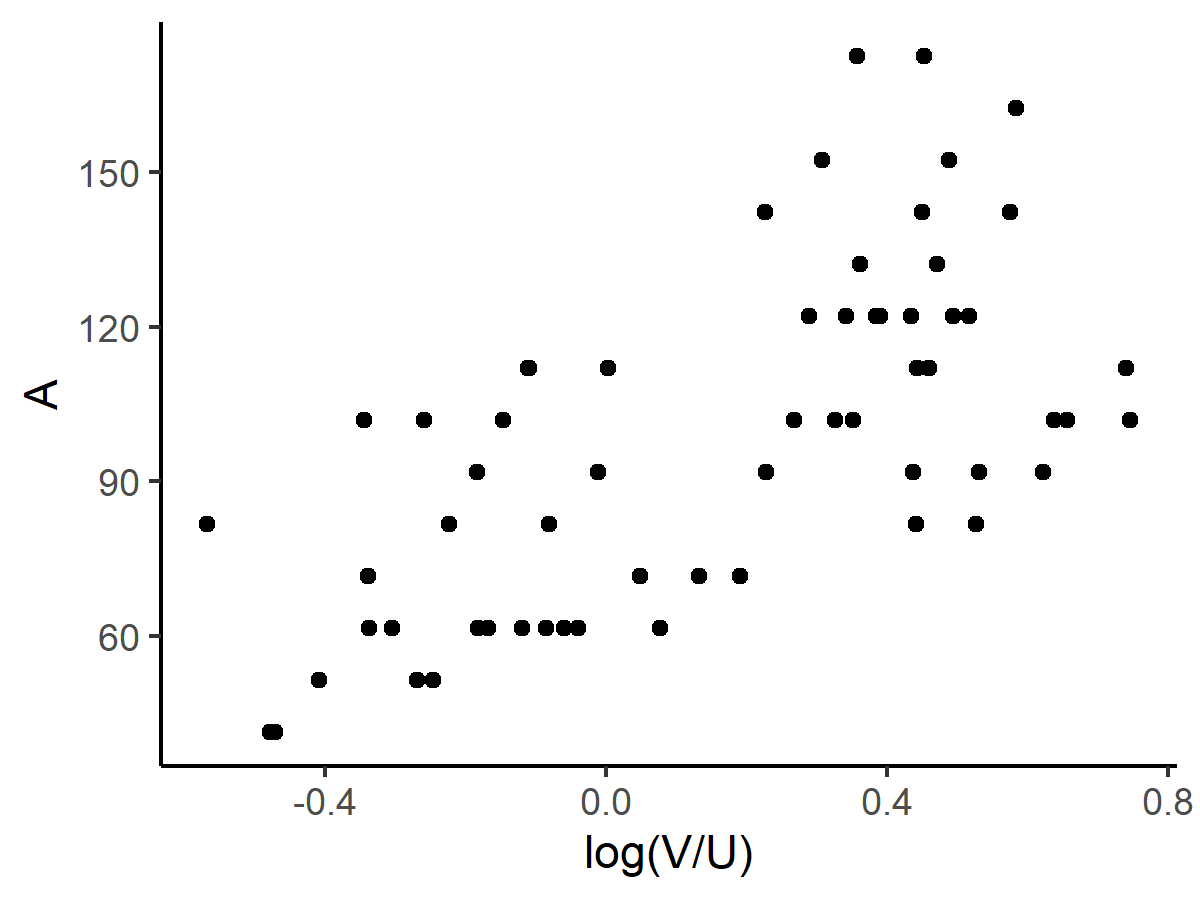
\includegraphics[width = 0.38\textwidth]
  {figuretable/efficiency_tightness_plot_year.png}}
  \caption{Year-level results}
  \label{fg:year_level_results} 
  \end{center}
  \footnotesize
  %Note: 
\end{figure} 



\begin{itemize}
    \item 
    \item The (logarithm of) job finding rate ($H/U$) and labor market tightness ($V/U$) like Figure 1 of \cite{borowczyk2013accounting}
    
\end{itemize}

\subsection{Month-level trends in 1966-2023}

Figure \ref{fg:month_level_results}

\begin{figure}[!ht]
  \begin{center}
 \subfloat[Unemployed ($U_{t}$) and Vacancy ($V_{t}$)]{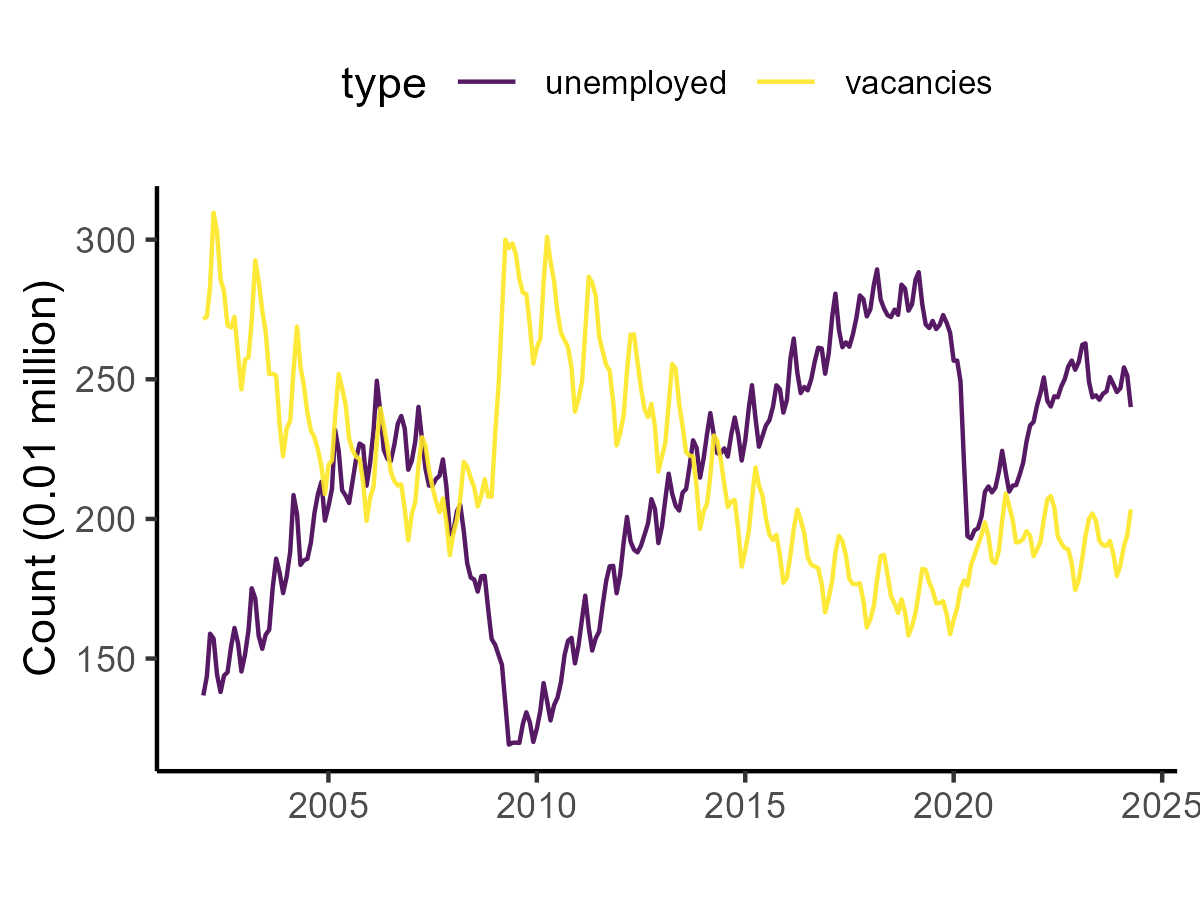
\includegraphics[width = 0.38\textwidth]
  {figuretable/unemployed_vacancy_month.png}}
  \subfloat[Hire ($H_{t}$)]{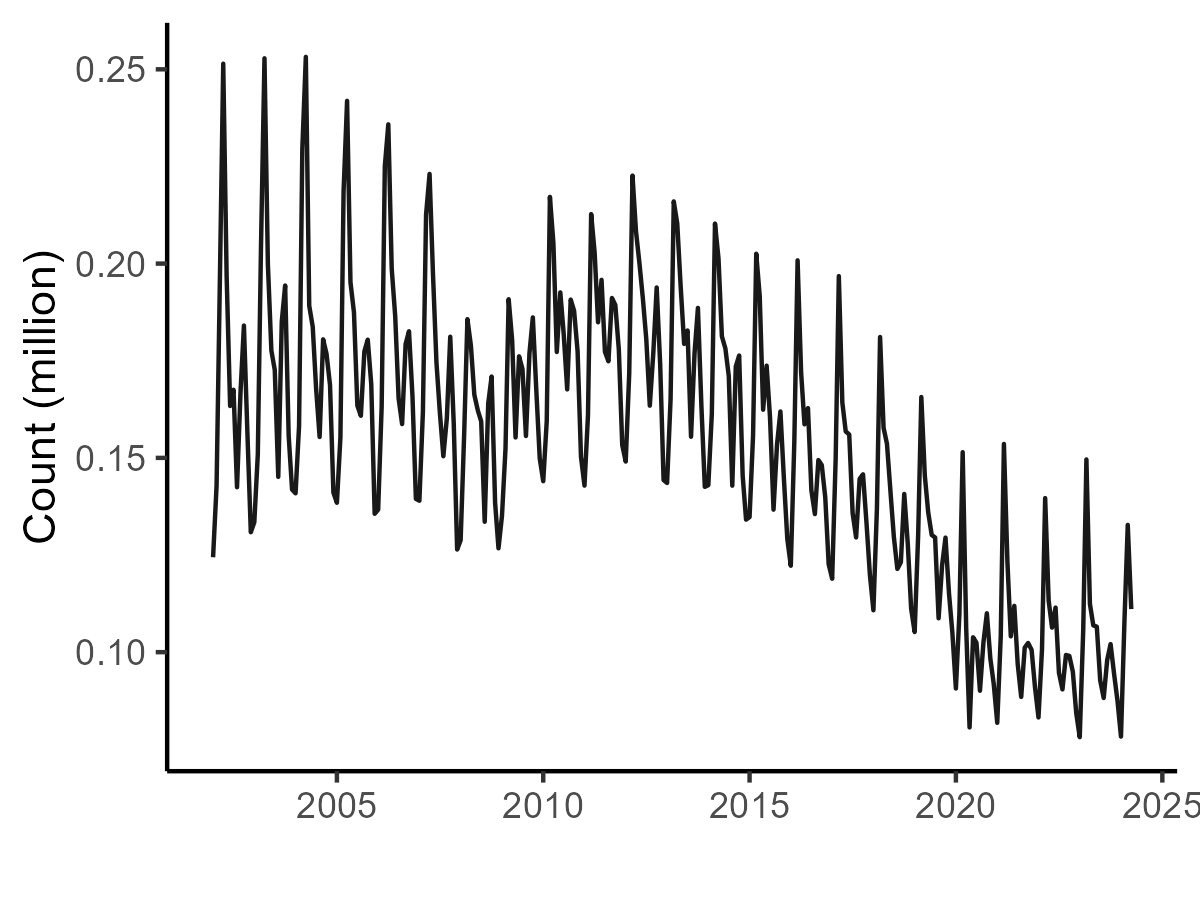
\includegraphics[width = 0.38\textwidth]
  {figuretable/hire_month.png}}\\
  \subfloat[Bevaledge Curve ($U_{t}$ and $V_{t}$)]{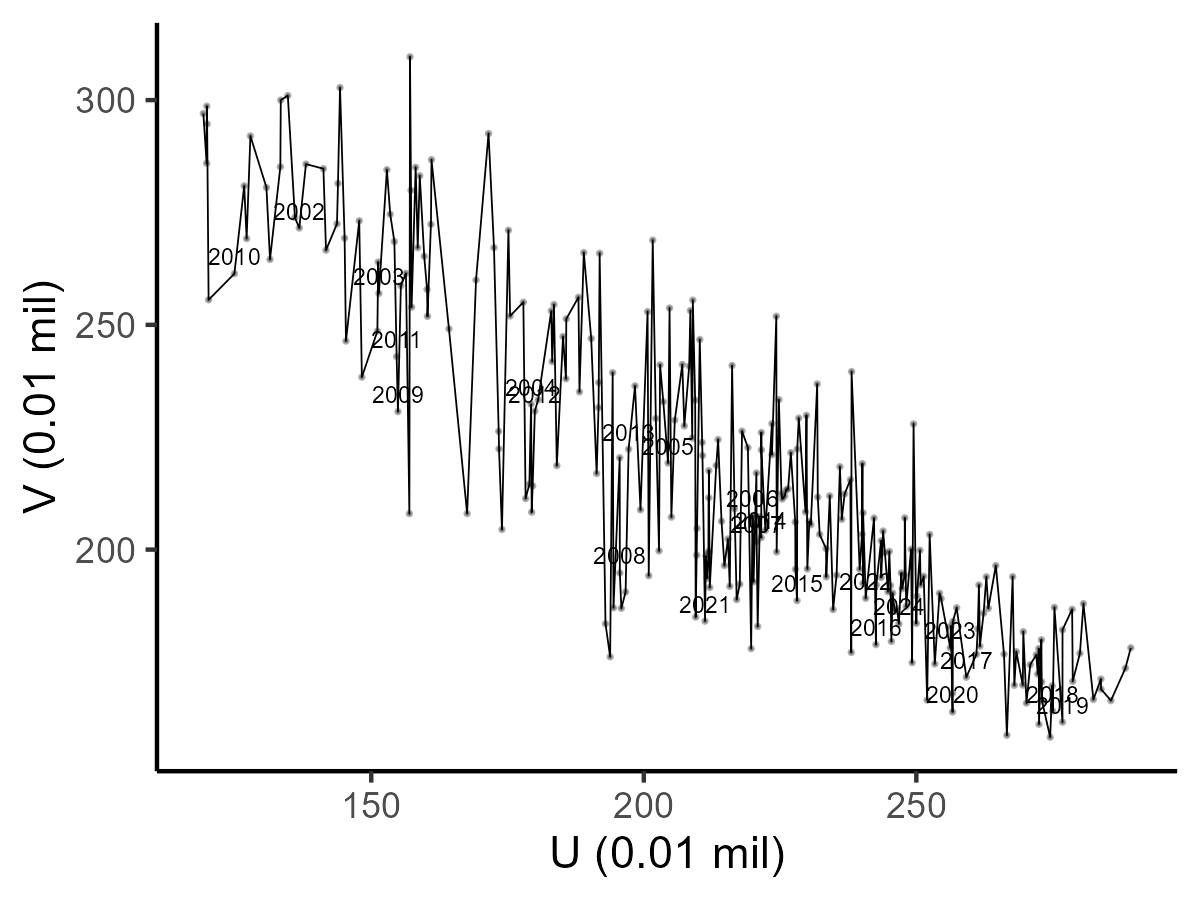
\includegraphics[width = 0.38\textwidth]
  {figuretable/unemployed_vacancies_berveridge_month.png}}
  \subfloat[Log job finding rate and tightness]{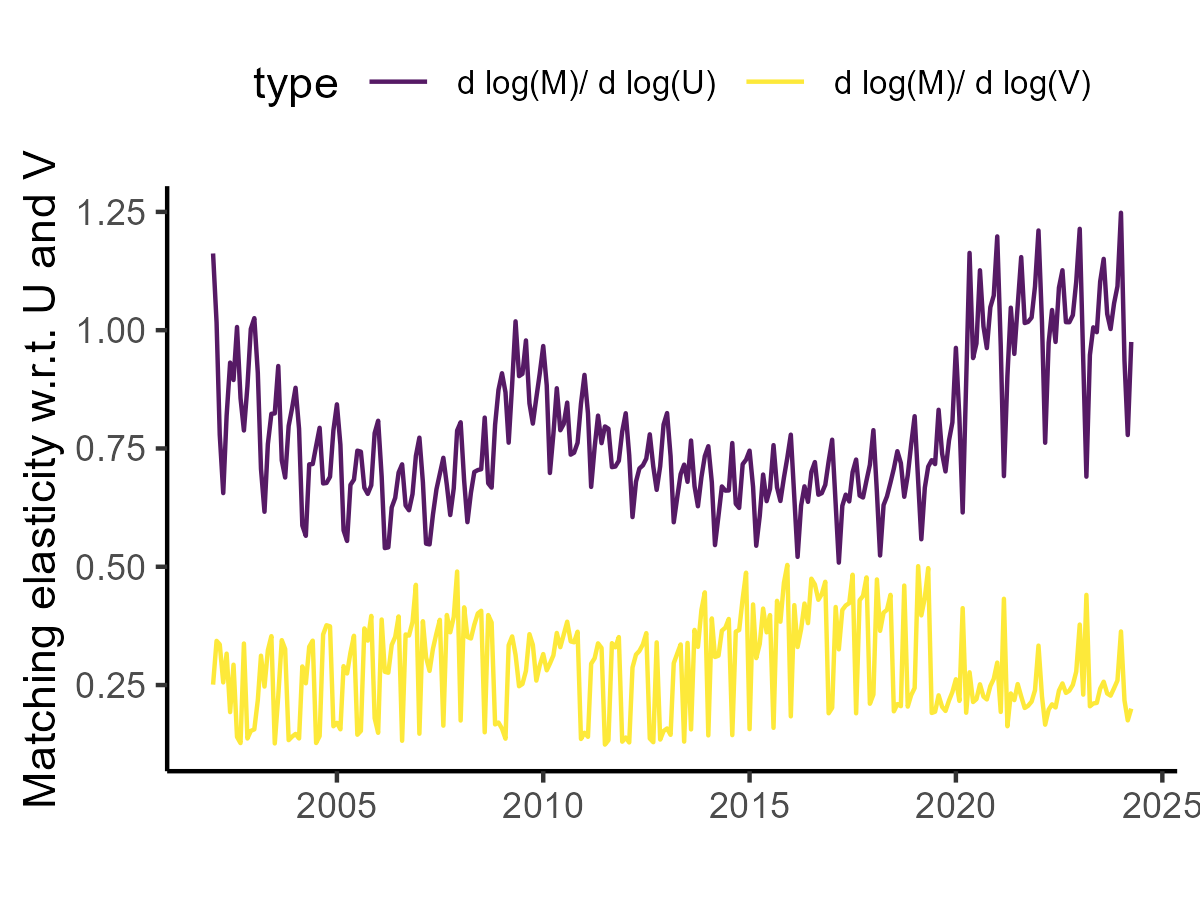
\includegraphics[width = 0.38\textwidth]
  {figuretable/elasticity_month.png}}
  \\
  \subfloat[Matching Efficiency ($A_{t}$)]{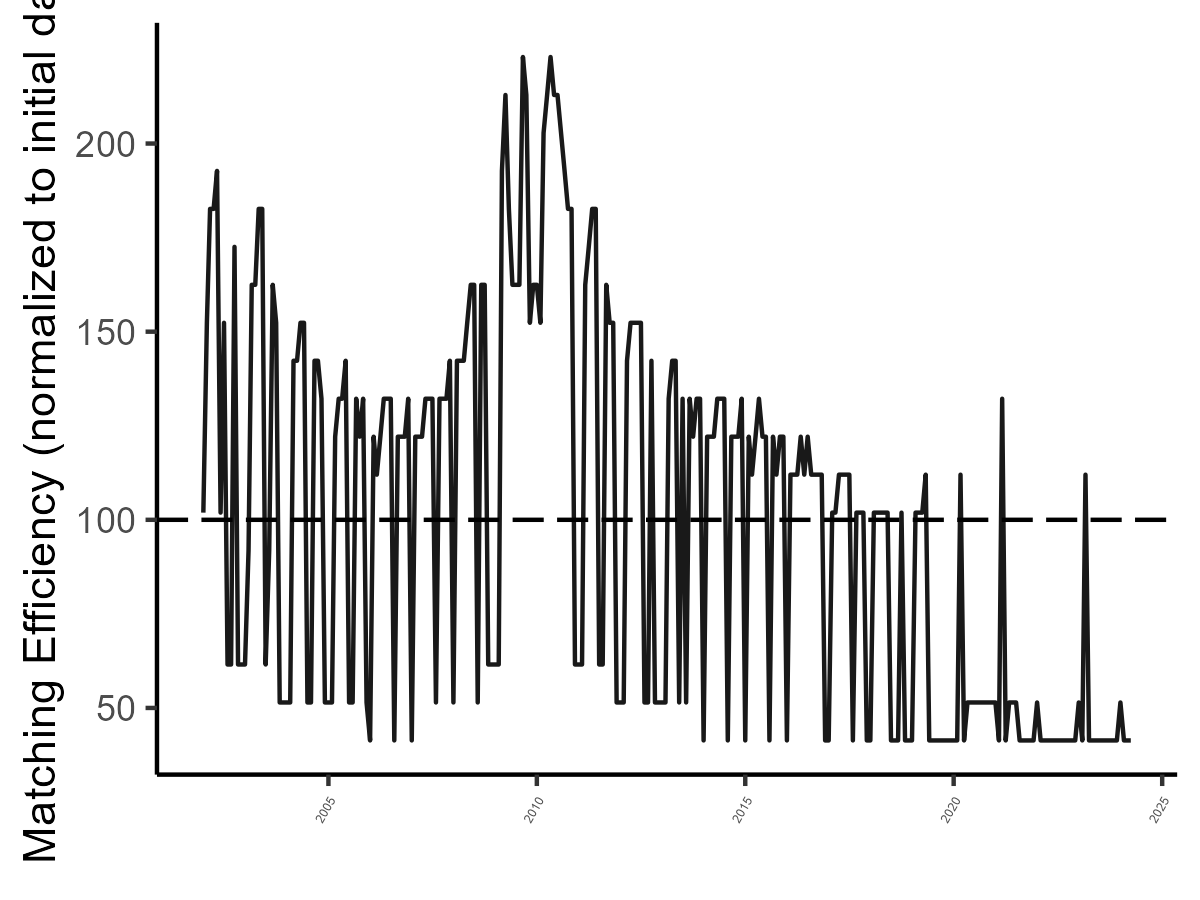
\includegraphics[width = 0.38\textwidth]
  {figuretable/matching_efficiency_month.png}}
  \subfloat[Matching Elasticity ($\frac{dM}{dU}$ and $\frac{dM}{dV}$)]{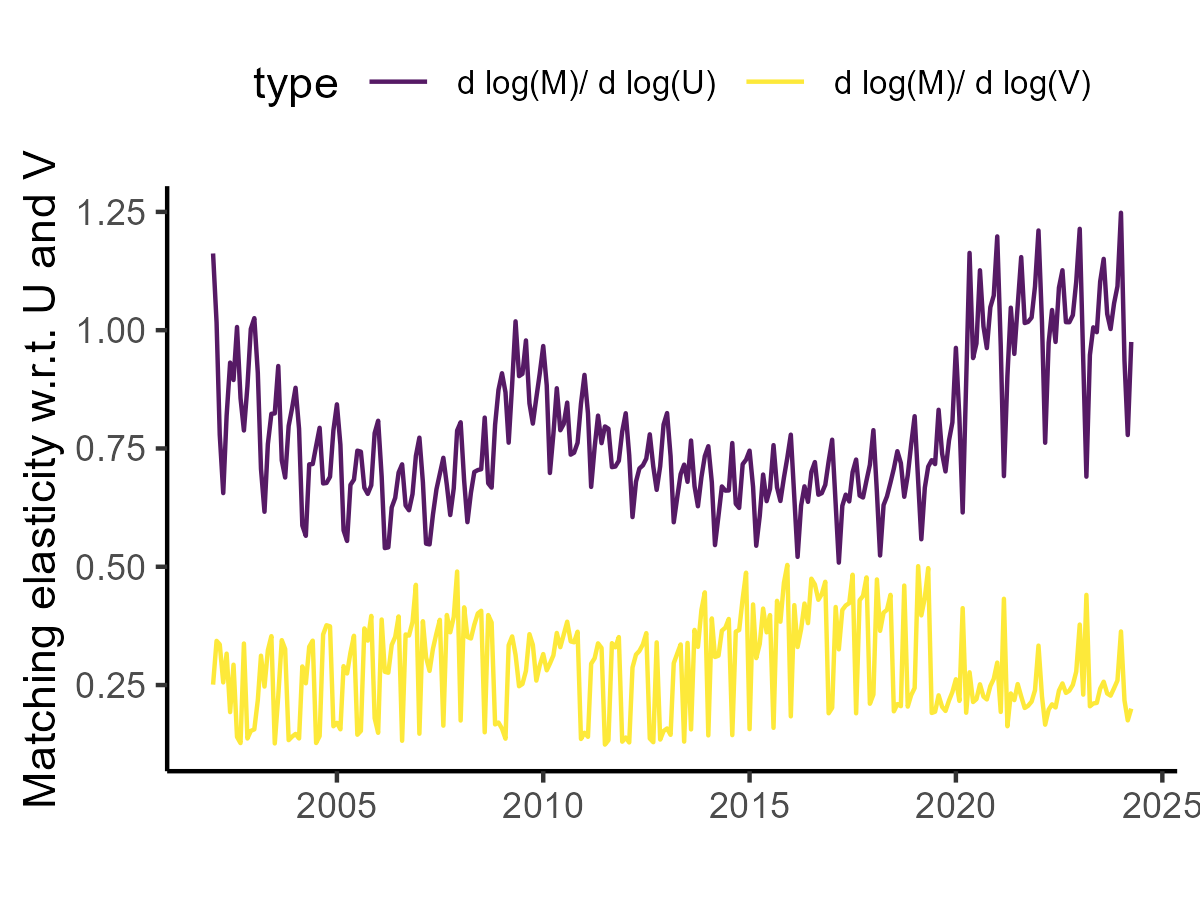
\includegraphics[width = 0.38\textwidth]
  {figuretable/elasticity_month.png}}\\
  \subfloat[Efficiency ($A$) and Tightness ($V/U$)]{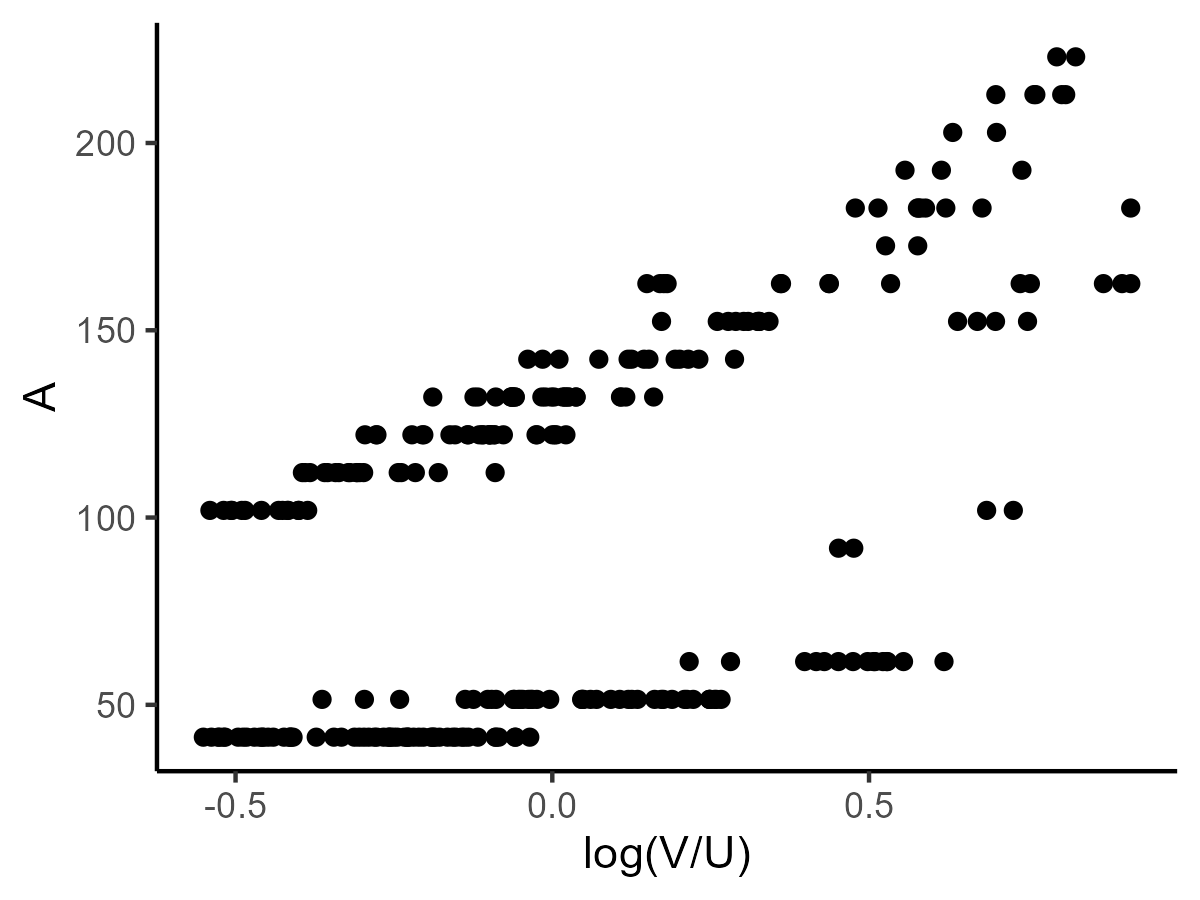
\includegraphics[width = 0.38\textwidth]
  {figuretable/efficiency_tightness_plot_month.png}}
  \subfloat[Efficiency ($A$) and job finding rate ($M/U$)]{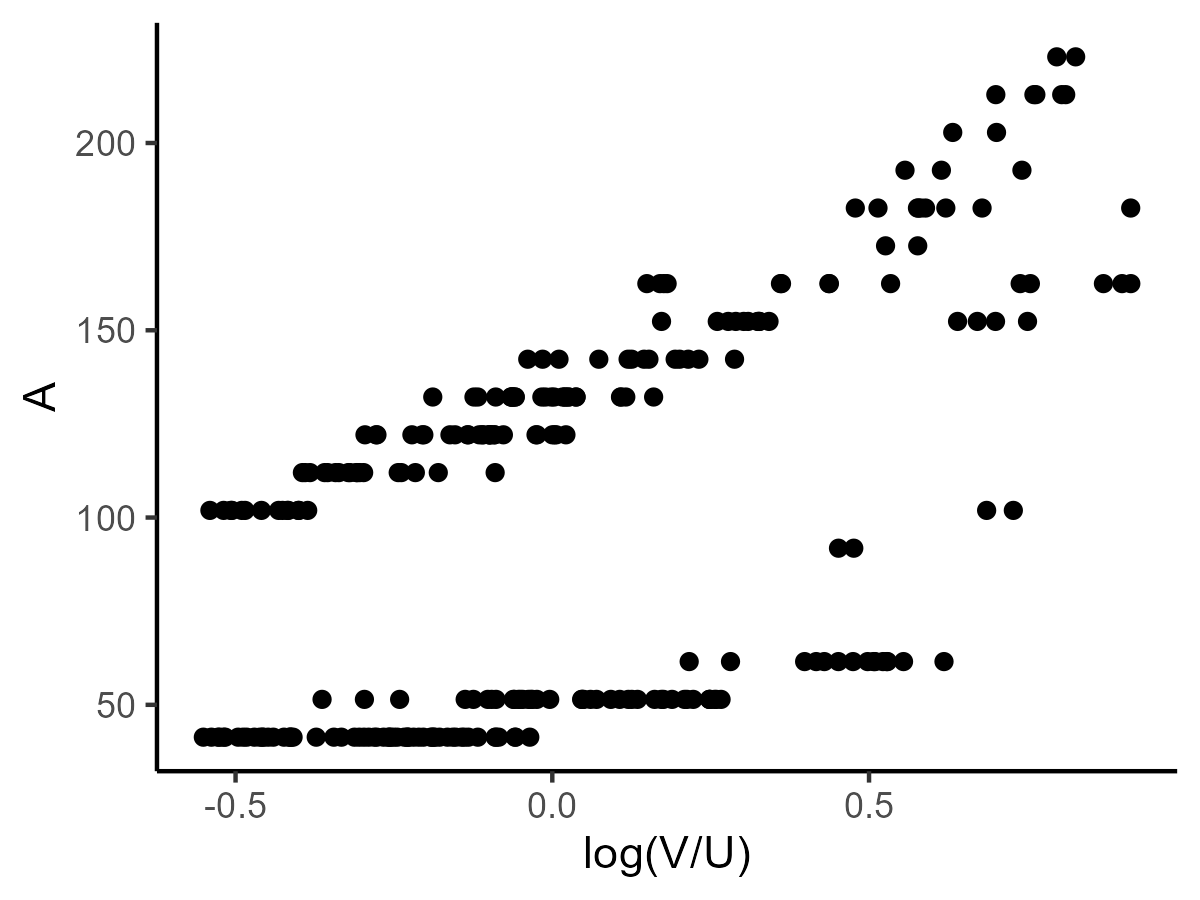
\includegraphics[width = 0.38\textwidth]
  {figuretable/efficiency_tightness_plot_month.png}}
  \caption{Month-level results}
  \label{fg:month_level_results} 
  \end{center}
  \footnotesize
  %Note: 
\end{figure} 

\begin{itemize}
    \item The (logarithm of) job finding rate ($H/U$) and labor market tightness ($V/U$) like Figure 1 of \cite{borowczyk2013accounting}
    
\end{itemize}

\section{Conclusion}


\paragraph{Acknowledgments}



\bibliographystyle{ecca}
\bibliography{matching_function}

\end{document}









